\documentclass[titlepage, a4paper]{article}
\usepackage[swedish]{babel}
\usepackage[utf8]{inputenc}
\usepackage{graphicx}
\usepackage{color}
\usepackage{mathtools}
\usepackage{etoolbox}

% Sidformat
\usepackage{a4wide}

% Bättre bildtexter
\usepackage[margin=10pt,font=small,labelfont=bf,labelsep=endash]{caption}

% Enkelt kommando som låter mig attgöra-markera text
\newcommand{\todo}[1] {\textbf{\textcolor{red}{#1}}}

\usepackage{graphicx,epstopdf}
\usepackage{listings}
\epstopdfsetup{suffix=}
\DeclareGraphicsExtensions{.ps}
\DeclareGraphicsRule{.ps}{pdf}{.pdf}{`ps2pdf -dEPSCrop -dNOSAFER #1 \noexpand\OutputFile}

\lstset{literate=%
    {å}{{\r{a}}}1
    {ä}{{\"a}}1
    {ö}{{\"o}}1
    {Å}{{\r{A}}}1
    {Ä}{{\"A}}1
    {Ö}{{\"O}}1
}

%% Headers och Footers
\usepackage{fancyhdr}
\pagestyle{fancy}
\rhead{Martin Söderén \\ Alexander Yngve}
\chead{TANA21}

\begin{document}

{\ }\vspace{45mm}

\begin{center}
    \Huge \textbf{TANA21: Projektrapport}
\end{center}
\begin{center}
    \Large Volymen på ett föremål
\end{center}

\vspace{250pt}

\begin{center}
    \begin{tabular}{|*{3}{p{40mm}|}}
        \hline
        \textbf{Namn} & \textbf{Personnummer} & \textbf{Epostaddress} \\ \hline
        {Martin Söderén} & {900929-1098} & {marso329@student.liu.se} \\ \hline
        {Alexander Yngve} & {930320-6651} & {aleyn573@student.liu.se} \\ \hline
    \end{tabular}
\end{center}
\newpage

\section{Inledning}
Projektets uppgift är att uppskatta volymen på ett oregelbundet föremål, exempelvis en sten eller en barkbit. Därefter ska felen i uppskattningen bedömas, det totala felet beräknas och antalet signifikanta siffror anges.

\section{Metod}\label{sec:metod}
Föremålet som valdes är stenen i figur \ref{fig:sten}.

\begin{figure}[h]
  \centering
  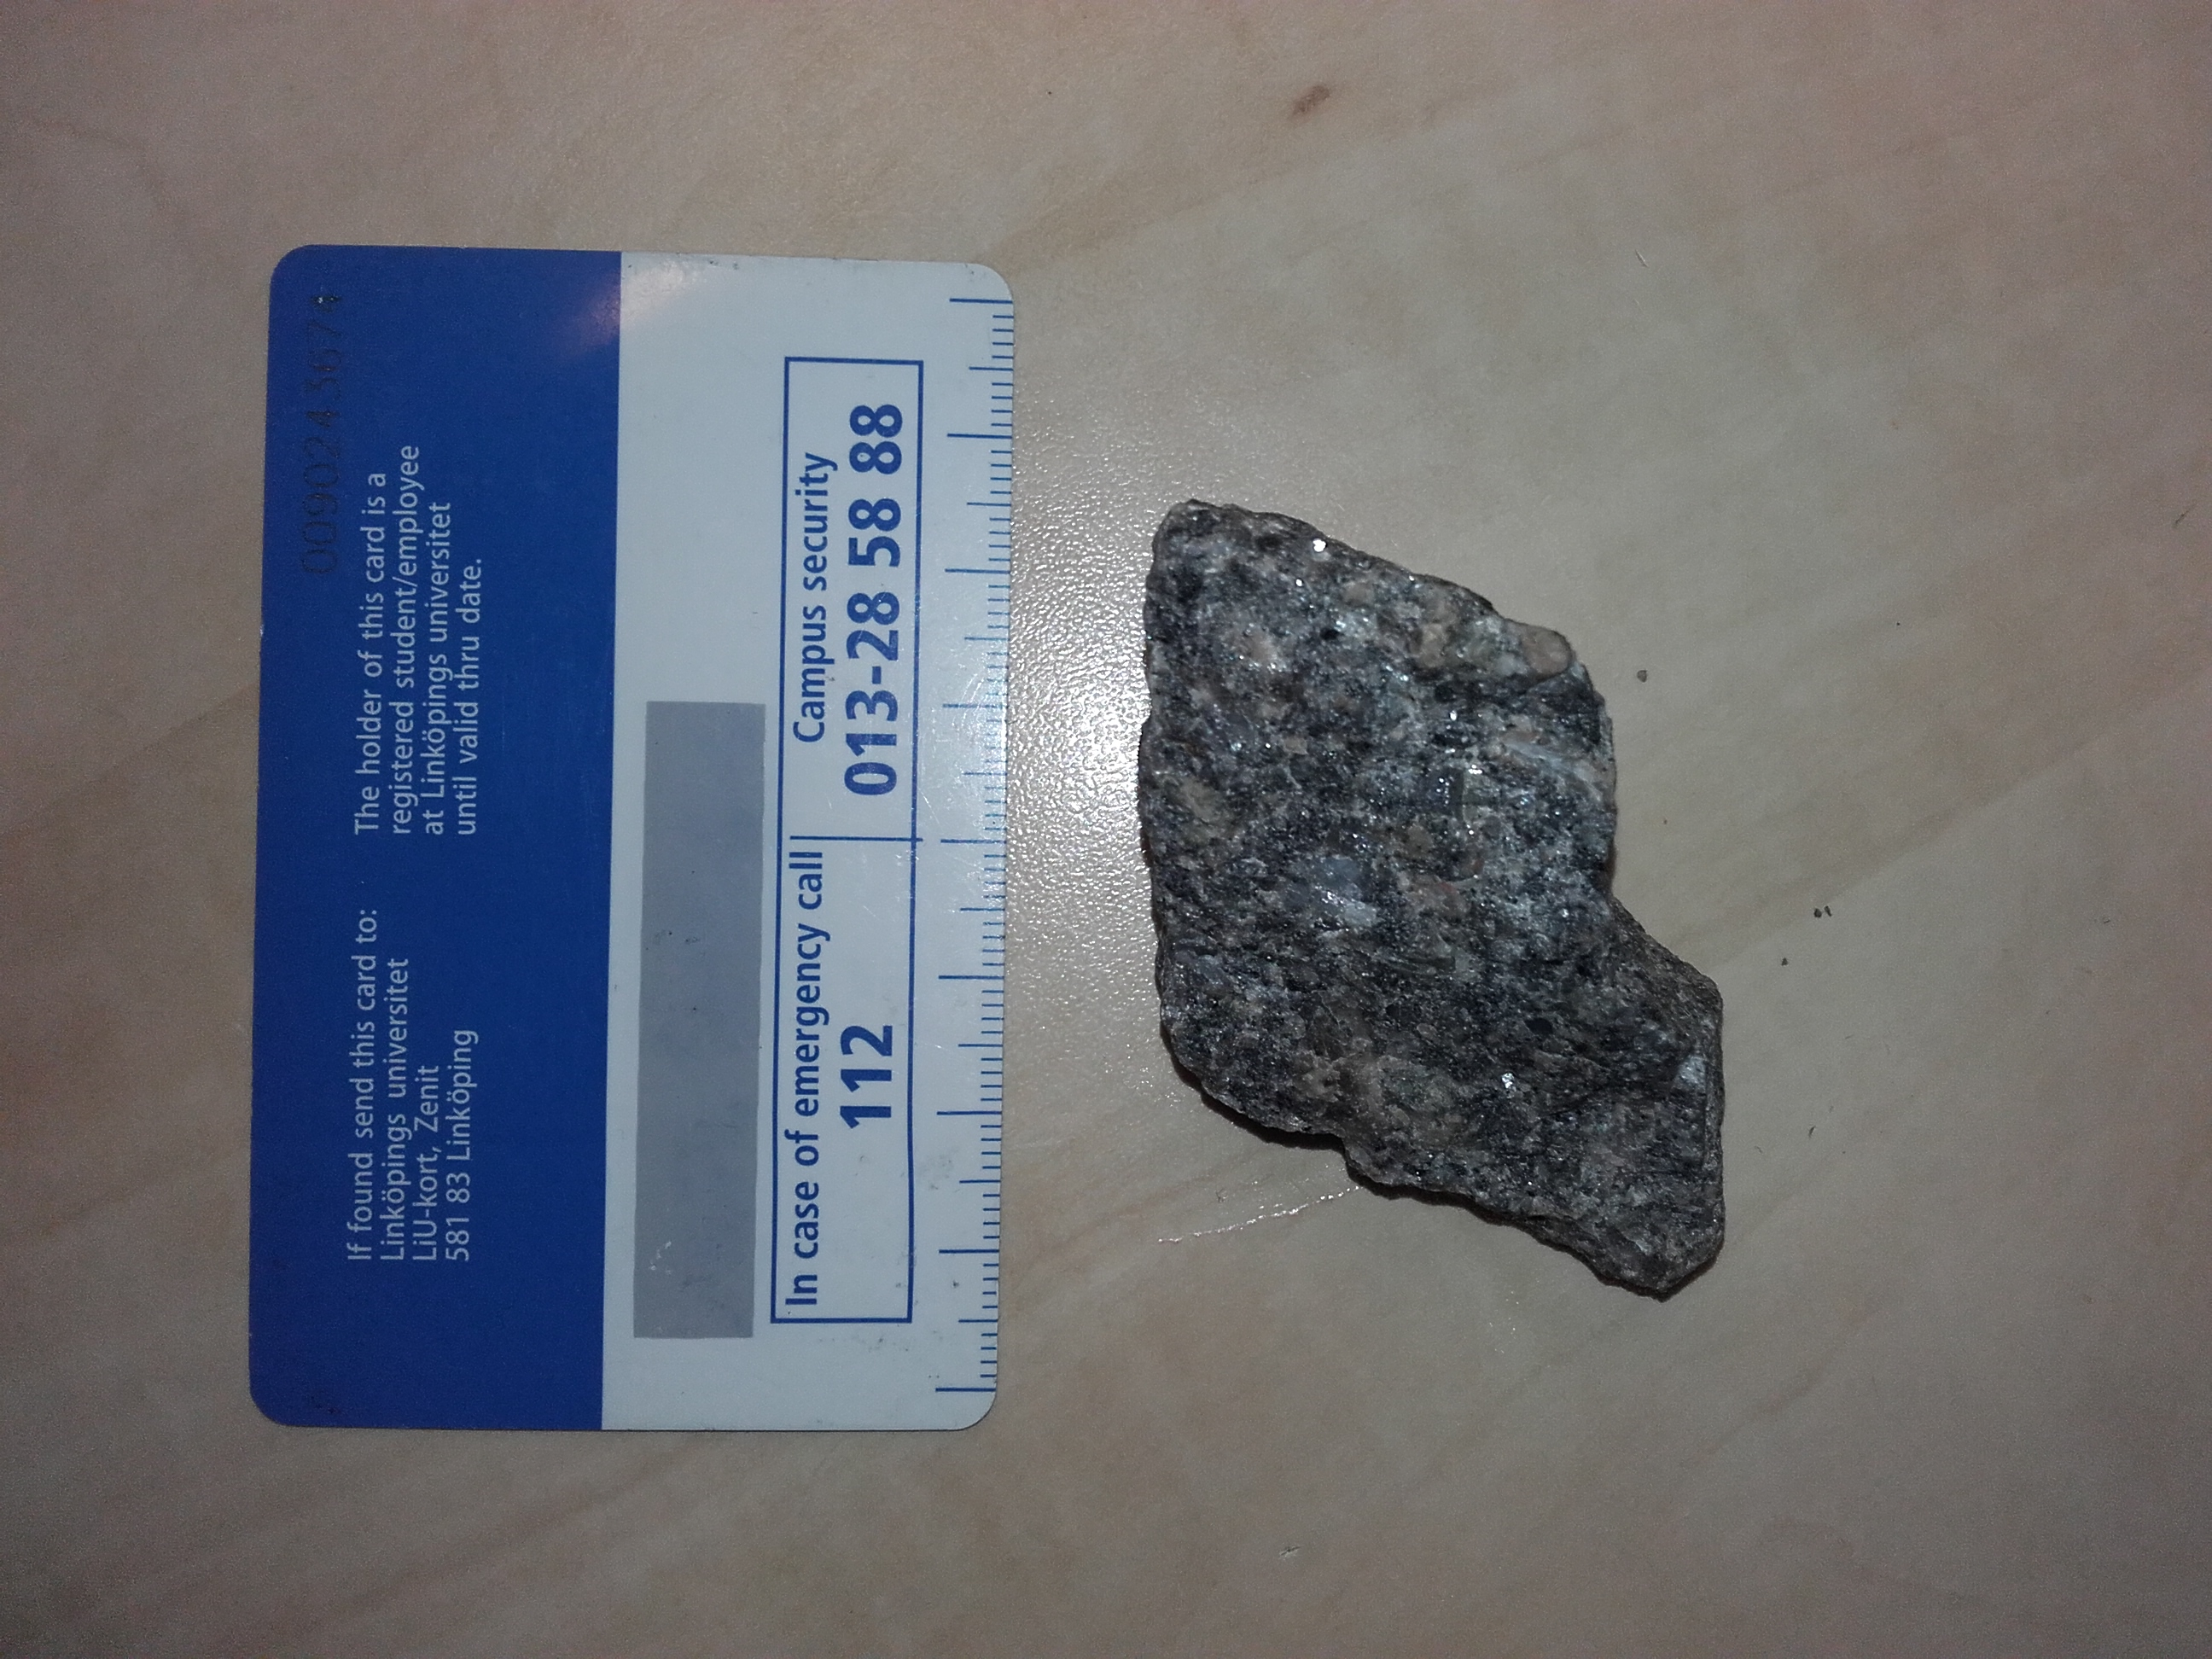
\includegraphics[scale=0.1]{grafik/sten.jpg}
  \caption{Stenen vars volym uppskattades.}
  \label{fig:sten}
\end{figure}

Volymen på stenen uppskattades genom att sänka ner stenen i en cylindrisk bägare med vatten och observera skillnaden i vattennivån. Volymen av en cylinder ges av $V=\pi r^2h$, där $r$ är radien och $h$ är höjden. Om $V_1$ och $h_1$ är vattnets volym och nivå i den cylindriska bägaren innan stenen sänks ner och $V_2=V_1 + V_{sten}$ och $h_2$ är volymen respektive vattennivån efter stenen sänks ner blir $V_2 - V_1 = \pi r^2h_2 - \pi r^2h_1 \Leftrightarrow V_{sten} = \pi r^2(h_2 - h_1)$.

Maximalfeluppskattningen för volymen $V_{sten}$ blir då $|\Delta V_{sten}| = |2\pi \bar{r}(\bar{h_2} - \bar{h_1})\Delta r| + |\pi \bar{r}^2\Delta h_1| + |\pi \bar{r}^2\Delta h_2|$, där $\bar{r}$, $\bar{h_1}$ och $\bar{h_2}$ är närmevärdet för respektive storhet.

$\bar{r}$, $\bar{h_1}$ och $\bar{h_2}$ mättes med skjutmått. Då det är lättare att mäta diameter än radie på en cylinder mättes det istället, det vill säga  $\bar{r} = \frac{\bar{d}}{2}$. Detta medför att felet $\Delta r$ halveras.

\section{Resultat}
Tabell \ref{tab:storheter} visar de uppmätta storheterna. Skjutmåttet som användes har en tolerans på $\pm 0,00005$ m. Detta ger $\Delta r = \pm 0,000025$, $\Delta h_1 = \pm 0,00005$ och $\Delta h_2 = \pm 0,00005$.

\begin{table}[h]
  \centering
  \begin{tabular}{|l|l|l|}
    \hline
    \textbf{Storhet} & \textbf{Värde} & \textbf{Enhet}\\ \hline
    $\bar{r}$ & 0,0400 & m\\ \hline
    $\bar{h_1}$ & 0,0350 & m\\ \hline
    $\bar{h_2}$ & 0,0404 & m\\ \hline
  \end{tabular}
  \caption{Uppmätta storheter.}
  \label{tab:storheter}
\end{table}

\clearpage
Enligt formlerna i avsnitt \ref{sec:metod} blir då närmevärdet för stenens volym samt maximalfeluppskattningen $\bar{V}_{sten} = 2,714*10^{-5} \text{m}^3$ respektive $|\Delta V_{sten}| = 0,05366*10^{-5} \text{m}^3$. Antalet signifikanta siffror är en eftersom antalet korrekta decimaler är fem. Volymen avrundas därför neråt till $\bar{V}_{sten} = 2,7*10^{-5}$ vilket introducerar avrudningsfelet $R_B = 0,014*10^{-5}$. Svaret är således $\bar{V}_{sten} = 2,7*10^{-5} \text{m}^3$ med ett totalt fel på $|\Delta V_{sten}| = 0,06766*10^{-5} \text{m}^3$.

\end{document}

